\section{Proxy Setup}
We want to setup a \textbf{proxy service} at \textbf{proxy.acme.group27} that can be exploited only by \textit{authenticated} users located in the \textit{Clients} subnetwork. For the sake of simplicity, the users we will accept and authenticate are the same we have defined previously for the \textbf{road warriors} set.\\
The setup is carried out entirely in the \textbf{proxy.acme.group27} machine, and even if this machine gives us the chance to setup an \textit{HTTP Squid Proxy service} through \textbf{zentyal} administration panel, we decide to setup \textbf{Squid} directly via the \textit{squid.conf} file as pictured in \textbf{Figure 4} (next page).\\
We decide to implement a \textbf{non-transparent proxy} given the requirements for the service, so that the users in the \textit{Clients} subnet will have to manually configure their browsers.\\
The service can be accessed, as anticipated in the previous assignment, on port \textbf{3128} via \textbf{HTTP}. Apart from defining several default \textbf{acl}s for different safe ports, we define an \textbf{acl} named \textbf{Clients$\_$net} to identify the target \textit{Clients} subnetwork, and an \textbf{acl} named \textbf{authenticated} which identifies users that have been successfully \textbf{authenticated} through module \textbf{basic$\_$ncsa$\_$auth} (\textbf{Figure 5}).\\
Notice that every user-password pair is stored under the file \textit{$/$etc$/$squid$/$passwd}, this and the whole authentication procedure will be discussed on the next paragraph.\\
At this point, with line \textit{http$\_$access allow Clients$\_$net authenticated} we grant access to users that are in the desired internal subnet and that have been successfully authenticated. Every other connection is denied through default line \textit{http$\_$access deny all}, and reply access is allowed if not denied before as default.\\
As pictured in the detail on \textbf{Figure 6}, as requested by the assignment the \textbf{proxy service} holds a \textbf{cache} and \textbf{log file} for it, as well as an \textbf{access.log} file to log all the accesses and operations performed by the authenticated users.\\
The firewall rules were already setup so that this service could be available from the \textit{Clients} subnetwork and so that its machine had Internet access. So, in order to visit one of white-listed websites - \textbf{cybersecurity.uniroma1.it} which has IP address \textbf{151.100.17.12} - we only need to start the daemon of the \textbf{Squid} service via command \textit{systemctl start squid} after having it enabled, and then setup the \textit{Firefox Browser} on the Kali machine so that it knows how to contact the service: \textit{Firefox $->$ Preferences $->$ Network Settings $->$ Settings $->$ Manual proxy configuration} with the very well known values (100.100.6.3 and 3128 as port) to be exploited with all protocols.\\
Results are showed in the sixth paragraph.\\

\begin{figure}[!htb]
\centering
\begin{minipage}{.33\textwidth}
  \centering
  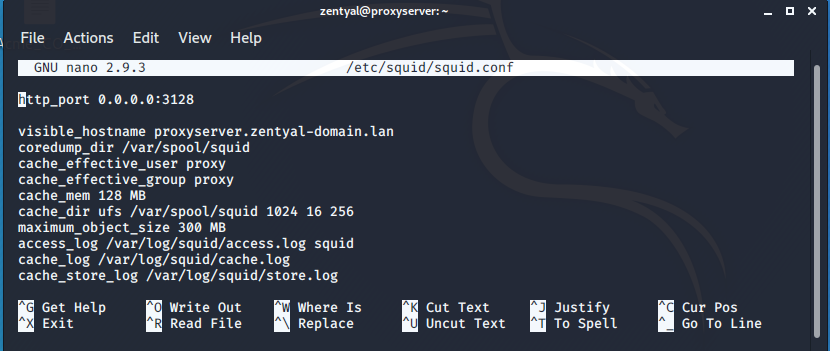
\includegraphics[width=1\textwidth]{squidConf1.png}
  \caption[a]{Beginning of the squid.conf file with the 3128 port specified.}\label{fig:4}
\end{minipage}%
\begin{minipage}{.33\textwidth}
  \centering
  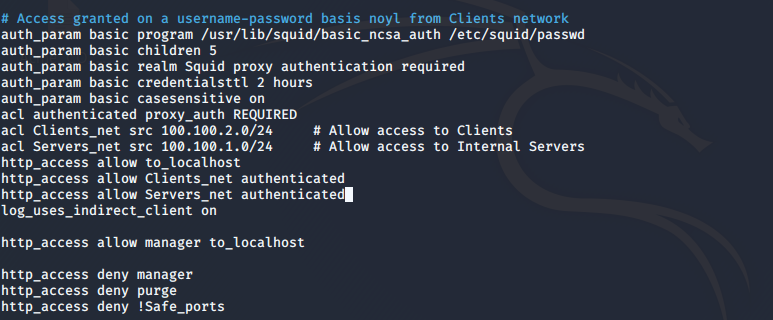
\includegraphics[width=1\textwidth]{squidConf2.png}
  \caption[a]{acls defined to restrict the access to the service.}\label{fig:5}
\end{minipage}
\begin{minipage}{.33\textwidth}
  \centering
  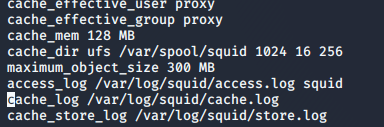
\includegraphics[width=1\textwidth]{squidConf3.png}
  \caption[a]{Configuring log files for cache and accesses to the service.}\label{fig:6}
\end{minipage}
\end{figure}
